%% \documentclass[conference,a4paper]{IEEEtran}
\documentclass[conference,a4paper,10pt]{IEEEtran}
\IEEEoverridecommandlockouts

% \usepackage{scrextend}
% \changefontsizes[20pt]{20pt}


% \usepackage{xcolor}

% \pagecolor{black}
% \color{white}


% ICCIT 2026 uses double-blind review. Add author details only for the camera-ready paper.

\usepackage{cite}
\usepackage{amsmath,amssymb,amsfonts}
\usepackage{graphicx}
\usepackage{textcomp}
\usepackage{xcolor}
\usepackage{booktabs}
\usepackage{tabularx}
\usepackage{array}
\usepackage{tikz}
\usepackage{url}
\usepackage{fancyhdr}
\usepackage[hidelinks]{hyperref}
\usetikzlibrary{arrows.meta,calc,fit,positioning,decorations.pathreplacing}
\urlstyle{same}

\setlength{\dbltextfloatsep}{13pt plus 2pt minus 2pt}

% ICCIT camera-ready notices appear only on the title page.
\fancypagestyle{iccitfirstpage}{%
  \fancyhf{}%
  % Keep the two-line notice in the existing header area.
  \fancyhead[L]{\footnotesize\raisebox{0pt}[0pt][0pt]{\shortstack[l]{%
    2026 29th International Conference on Computer and Information Technology (ICCIT)\\
    18-20 December 2026, Cox's Bazar, Bangladesh}}}%
  \fancyfoot[L]{\footnotesize
    979-8-3195-0171-4/26/\$31.00~\copyright{}2026 IEEE}%
  \renewcommand{\headrulewidth}{0pt}%
  \renewcommand{\footrulewidth}{0pt}%
}
\pagestyle{empty}

\definecolor{jbblue}{RGB}{35,91,133}
\definecolor{jbteal}{RGB}{35,116,105}
\definecolor{jbamber}{RGB}{171,106,29}
\definecolor{jbred}{RGB}{158,48,48}
\definecolor{jbgray}{RGB}{241,243,245}
\definecolor{jbink}{RGB}{39,50,56}

\def\BibTeX{{\rm B\kern-.05em{\sc i\kern-.025em b}\kern-.08em
    T\kern-.1667em\lower.7ex\hbox{E}\kern-.125emX}}

\begin{document}

\title{Islands of Reach: A Censorship-Resistant Federated Forum for
National Internet Blackouts}

\author{%
  \IEEEauthorblockN{Tasmir Hossain Zihad\quad Sarwad Hasan Siddiqui\quad Rezuan Mustafa Hasan}
  \IEEEauthorblockA{Khulna University of Engineering \& Technology\\
    Khulna 9203, Bangladesh\\
    \texttt{tasmir@tuta.io}\quad \texttt{sarwad015@gmail.com}\quad
    \texttt{hasanideal2002@gmail.com}}
}

\maketitle
\thispagestyle{iccitfirstpage}

\begin{abstract}
  An Internet shutdown is rarely a clean power switch. Transit to the outside world can be withdrawn while domestic networks keep carrying packets among themselves, leaving reachable fragments that recent measurement work calls connectivity islands. We ask a narrow question: when some domestic IP paths survive, can independently operated forum servers keep accepting signed posts and reconciling them across whatever graph remains? Our prototype composes four familiar mechanisms for this regime: canonical protobuf envelopes admitted as the exact bytes their author signed, operator receipts bound to those bytes, caller-initiated synchronisation that survives asymmetric reachability, and an explicitly trusted dual-homed relay between islands. On a four-node testbed, all 20 dependency chains reached the destination in each route regime. Median post latency was 0.735 seconds with the exchange intact and 1.732 seconds via the bridge after the cut. An eight-node chain delivered all 50 envelopes to hop seven with a 2.368-second median at a 500-millisecond drain interval. TypeScript, Rust and Python agreed on 20,000 generated and mutated envelope cases. With inbound connections blocked, periodic pull recovered all 10 posts, while the minimal ActivityPub push baseline delivered none. These results establish partition tolerance under surviving IP paths on a single-host testbed, and nothing about total blackouts, real inter-provider deployment, or resourced denial of service.
\end{abstract}

\begin{IEEEkeywords}
  federated systems, Internet shutdowns, network partitions, signed objects, store-and-forward
\end{IEEEkeywords}

\section{Introduction}

An Internet shutdown does not necessarily mean a complete loss of connectivity. Disruptions can reduce bandwidth, block destinations, filter protocols, or withdraw international routes \cite{ooni2025bangladesh}. Despite these restrictions, domestic networks can still communicate with each other \cite{bischof2023shutdowns,baltra2024connectivity}. Baltra et al. call networks that lose access to the Internet core while retaining local connectivity “islands” \cite{baltra2024connectivity}. They call networks with partial reachability “peninsulas.” We ask whether independently operated forum servers can receive signed posts and synchronize them across surviving domestic IP paths.

Circumvention systems are designed to reach a blocked region. Snowflake, for instance, routes a blocked user out through temporary proxy servers \cite{bocovich2024snowflake}. Such systems need a reachable proxy or cooperating network infrastructure. Anix, Rangzen and Moby instead construct a device-to-device or mobile mesh network for situations where general internet access is unavailable \cite{kamali2025anix,lerner2016rangzen,pradeep2022moby}. We examine whether independent servers can continue to check, store and relay messages over surviving domestic IP paths.

This paper makes four contributions:

\begin{enumerate}
  \item The server follows the same byte-preserving admission process for local and federated objects.
  \item Caller-initiated delivery, streaming and backfill let a server publish and recover objects over outbound connections to known peers.
  \item A quota-bounded relay validates each object, applies quotas and excludes the sending peer from fan-out. Trust governs quota and traffic classes. The same validity rules apply to all peers.
  \item The testbed evaluates route cuts, network impairments, hop scaling, admission under load, and delivery against a minimal ActivityPub inbox. Cross-language tests check the wire format.
\end{enumerate}

Our claim is limited to partition tolerance only when some IP paths remain between servers directly or through a bridge. This design cannot create a new route during complete blackout. This cannot force a server to accept a valid post or hide any visible relay from its hosting network operator. The work addresses resilient networking and security in distributed systems. Fig.~\ref{fig:architecture} summarizes the roles and trust paths.

\begin{figure*}[!t]
  \centering
  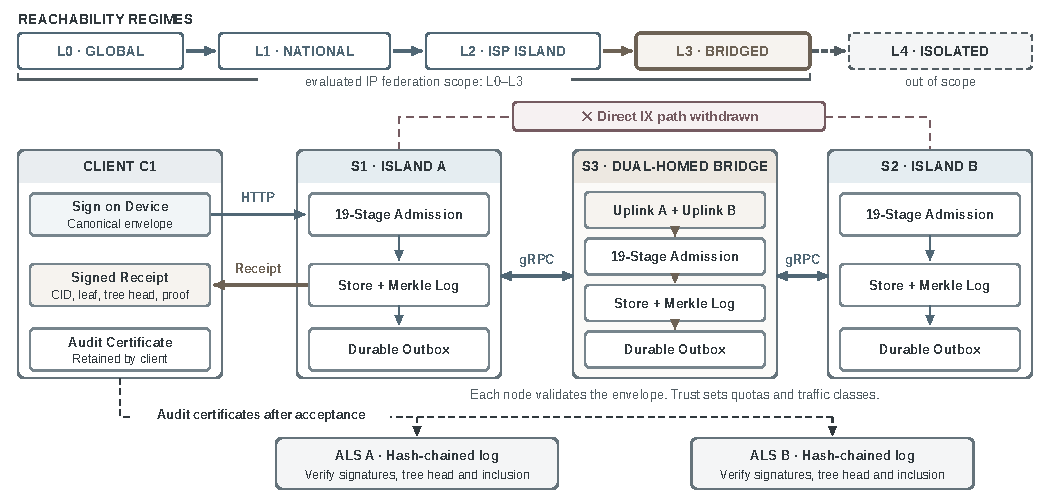
\includegraphics[width=\textwidth,trim=0 0 0 47bp,clip]{figures-v2/fig1-system-architecture-muted.pdf}
  \caption{System architecture: validating island nodes, a dual-homed bridge, and independent audit-log services.}
  \label{fig:architecture}
\end{figure*}

\section{Background and Research Gap}
\label{sec:background}

\subsection{Federated and Signed System}

ActivityPub directly delivers social activities to the server’s inbox \cite{activitypub}. AT protocol supports federation and repository replication \cite{atproto}. Nostr replicates objects signed by the author \cite{nostr}.  They generally assume that a relevant server, relay, or peer endpoint remains reachable. Our evaluation combines exact-byte admission, operator receipts, outbound recovery and relay policy between two network islands.

\subsection{Communication During Blackout}

Anix, Rangzen and Moby establish a network connecting nearby devices \cite{kamali2025anix,lerner2016rangzen,pradeep2022moby}. These systems can operate without a server connection. Our system requires a surviving IP path between servers. The two designs serve different connectivity conditions and workloads.

\subsection{Accountability}

Append-only logs, signed tree heads and inclusion proofs are defined by Certificate Transparency to make certain classes of misbehaviour auditable after the fact \cite{rfc9162}.  PeerReview and CoSi explore several stronger forms of accountability by using witnesses and cosigning \cite{haeberlen2007peerreview,syta2016cosi}. Our receipt proves that an operator acknowledged a specific content ID at a stated time. Delivery and refusals before admission fall outside this guarantee.

\subsection{Study gap and design objective}

Conventional server federation depends on reachable endpoints, while device-to-device systems can operate without Internet paths. We study an intermediate situation where independent servers can use surviving domestic paths after international routes are withdrawn. In this situation, our goal is to admit each signed object once per server, keep its signed bytes unchanged, and allow every reachable server using the same rules and prerequisite state to reach the same validity decision.

\section{System Design}
\label{sec:design}

\subsection{Architecture}

We designed a system that works as connectivity narrows while making server acceptance externally auditable. We model domestic exchange traffic surviving lost international transit and ISP islands joined by a dual-homed relay. Clients reach nodes over HTTP and nodes federate over gRPC; all claims are scoped to that surviving IP path.

The signed envelope is invariant across ingress and relay paths. Every node applies the same 19-stage pipeline: the first 12 stages validate without persistent writes; acceptance then commits the object, signs a receipt, and queues a durable federation task. The scheduler drains in priority and sequence order and batches by peer and plane. The bridge applies quotas by source uplink, destination uplink, and priority. Ingress kind, supplying peer, direction, uplink, traffic class, and quota policy govern deduplication, replay protection, scheduling, and fan-out, but never relax signature, identifier, or body validation.

The dual-homed bridge runs the same validating stack rather than transparently forwarding packets. Its relay capability is independently validated, stored, and quota-bounded under its own key.

Independent audit-log services (ALSs) sit outside the write path. After committing an object, the server returns a signed receipt; the client forms a public audit certificate, retains it, and forwards it to one or more ALSs. Each ALS checks canonical decoding, the author signature, the content and server identifiers, the receipt signature, the signed tree head, and the inclusion proof before appending the certificate to a hash-chained record. The acknowledgement therefore remains externally verifiable if the accepting server later hides or deletes the object, limiting its ability to erase evidence silently.

\subsection{Signed objects and admission}

An envelope carries a domain tag, an object type, a payload, a public key, a
nonce, and a creation timestamp. The receiver checks \texttt{created\_at\_ms} against a window from seven days before to ten minutes after its clock. Its identifier is the SHA-256 digest of a specified
canonical byte string, and an Ed25519 signature covers that same string
\cite{bernstein2012ed25519}. Protobuf does not guarantee a unique
serialisation \cite{protobufnotcanonical}, so we constrain a profile on top of
it (ascending field order, minimal varints, no unknown fields retained) and require that decoding and re-encoding an object
must reproduce the bytes as received, exactly. An object that fails that
comparison is rejected outright, never repaired.

Verifying the exact received bytes after a strict decode is established practice in DER, JWS, and Certificate Transparency leaf formats \cite{rfc9162}. In this system, the rule protects federation. If a relay decoded a peer’s bytes and re-encoded them before checking the signature, it could normalise a non-canonical submission into the canonical form that was signed. The relay would then verify reconstructed bytes rather than the bytes that arrived. Our decode–re-encode comparison prevents a receiver from repairing or normalising attacker-controlled bytes before verification. As a result, no relay can make a non-canonical or invalid submission acceptable by rewriting it.

Fig.~\ref{fig:pipeline} lays out the admission path. Stages 1 through 12 (size, parsing, canonicality, domain separation, identifier derivation, signature, clock window, and replay) write nothing to persistent
storage. HTTP limits and gRPC quotas apply before admission. Stage 13 applies origin anti-abuse policy, stage 14 checks authorization, and stage 15 validates the payload. The node commits the raw object, indexes, and Merkle leaf in one transaction before enqueueing federation. Exact retries are made idempotent under concurrency by a
uniqueness constraint in the database, not by a read-then-write check that a
race could defeat.

\begin{figure}[!t]
  \centering
  {\normalsize
  \begin{tabularx}{\columnwidth}{@{}l>{\raggedright\arraybackslash}X@{}}
    \toprule
    \textbf{Stage} & \textbf{Check or action} \\
    \midrule
    Before stage 1 & HTTP rate limit or gRPC peer quota \\
    \midrule
    1--2 & Size, parse, canonical re-encoding \\
    3--7 & Version, domain, plane, size, algorithm, priority \\
    8--10 & Clock window, signature, certificate \\
    11--12 & Content-ID deduplication and nonce replay check \\
    \midrule
    13 & Origin anti-abuse policy \\
    14--15 & Authorization and semantic validation \\
    16--18 & Atomic storage, projection, Merkle append, and signed receipt \\
    19 & Durable fan-out to eligible peers \\
    \bottomrule
  \end{tabularx}}
  \caption{Admission pipeline for local and federated envelopes. Entry quotas precede the read-only checks and authorization occurs at stage 14.}
  \label{fig:pipeline}
\end{figure}

On acceptance, the server signs a receipt binding the content identifier, the
leaf position, the resulting signed tree head, and an inclusion proof. The
acknowledgement therefore commits to the exact bytes admitted. Peers also exchange signed tree heads containing
a tree size, root hash, and timestamp. Two heads of equal size with different
roots are an unambiguous conflict. A larger head advances the stored observation. The gRPC exchange leaves its consistency unverified. A smaller
head is also not immediately treated as a fork, as observations may arrive out
of order: in case the timestamp is older than the recorded head, it is discarded as
stale; otherwise, a smaller size is reported as a possible fork. This is
deliberate stale-head handling. It removes a class of self-inflicted false
positives and catches outright tree shrinkage, however it is not full fork
detection. An adversary who rewrites history while keeping the tree size
non-decreasing can pass these local checks, and equivocation between two peers
cannot be detected by a single local comparison. Detecting those cases requires
consistency proofs and independent cross-observer exchange, which the network
partitions we target are likely to obstruct.

\subsection{Partition-aware federation}

Three caller-initiated RPCs cover ordinary delivery and recovery.
\textsc{Deliver} pushes a batch of accepted envelopes to a peer.
\textsc{StreamActivities} reads a finite snapshot from a durable cursor.
\textsc{Backfill} requests objects that the node knows it missed, using a
resumable log position. Because all three operations are initiated by the
caller, a node does not need to accept inbound federation connections. A
server behind carrier-grade NAT can therefore federate in both directions
over connections it opens itself. This solves reachability asymmetry, not
discovery: at least one peer address must already be known. A timer checks for catch-up every 2\,s. Outbound-only nodes poll known peers. Other nodes pull when inbound traffic is stale for two polling intervals.

The scheduler keeps an independent durable queue for each destination peer.
It drains these queues concurrently under bounded leases, with deadlines,
exponential backoff, and idempotency keys. Concurrent peer leases keep an unreachable peer from stalling the bridge. Delivery cancels its gRPC call after 15\,s by default. Control RPCs and backfill have 5\,s and 30\,s deadlines. Retry delays double from 1\,s to a 15\,min cap. The 13th failure dead-letters the entry after 47\,min 3\,s of backoff alone. Peer hints are capped at 60\,s. The testbed probes uplinks every 5\,s with a 1.5\,s timeout and a two-failure threshold.

Fig.~\ref{fig:topology} shows the route-cut topology used in the evaluation.
Island A contains two ordinary nodes, island B contains one, and a shared
exchange segment stands in for an Internet exchange point. The bridge holds
one address on each island network. Once the exchange segment is withdrawn,
both islands must already have configured trust in the bridge. That trust
determines the rate and priority of the bridge's traffic; it never determines
whether an envelope is valid. The bridge validates and stores every object it
relays, enforces quota per uplink pair and traffic class, and never sends an
object back to the peer from which it arrived.

\begin{figure}[t]
  \centering
  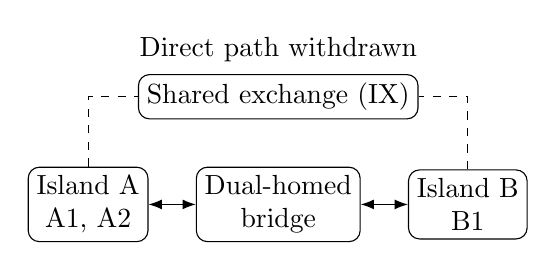
\begin{tikzpicture}[font=\normalsize, >=Latex, node distance=6mm,
      box/.style={draw, rounded corners, align=center, inner sep=3pt}]
    \node[box] (bridge) {Dual-homed\\bridge};
    \node[box, left=of bridge] (a) {Island A\\A1, A2};
    \node[box, right=of bridge] (b) {Island B\\B1};
    \node[box, above=of bridge] (ix) {Shared exchange (IX)};
    \draw[<->] (a) -- (bridge);
    \draw[<->] (bridge) -- (b);
    \draw[dashed] (a.north) |- (ix.west);
    \draw[dashed] (b.north) |- (ix.east);
    \node[above=1pt of ix] {Direct path withdrawn};
  \end{tikzpicture}
  \caption{Route-cut topology. The bridge connects the islands after withdrawal of the shared exchange.}
  \label{fig:topology}
\end{figure}

Federation passes the original envelope as opaque bytes. Push and backfill can race, so a database uniqueness constraint makes duplicate delivery idempotent. Trust determines quota and priority, and each relay applies the full admission checks.

\section{Methodology}
\label{sec:method}

We evaluate five questions: whether independent encoders agree on the
canonical form, whether objects cross an enforced route cut, how delivery
latency scales with hop count, whether malformed requests produce storage
writes, and how the representation compares in size with ActivityPub. All
experiments run on one physical host; \S\ref{sec:limits} treats the
consequences of that choice at length.

\textbf{Correctness tests.} TypeScript, Rust and Python run 16 positive reference vectors and a seeded differential suite of 10,000 valid and 10,000 mutated cases. The generators cover numeric boundaries, NFC Unicode, and empty anti-abuse fields across the valid corpus and 16 mutation classes. The suite compares canonical bytes, content identifiers, round trips, and decoder decisions. The authors' regression tests and fuzz corpus leave an independent security audit open.

\textbf{Route-cut experiment.} Four application nodes, two databases, and two
caches are distributed across three isolated virtual network segments, as
shown in Fig.~\ref{fig:topology}. Containers supply reproducible layer-2
isolation and let the harness withdraw the configured direct inter-island path
mid-run; nothing in the design depends on that packaging.

The test runs in four stages. It first reads kernel TCP state from \texttt{/proc/net/tcp} inside the bridge to confirm the local source address each established federation connection left from. It then withdraws the shared exchange segment and verifies that direct inter-island probes fail, and that island~B does not already hold the content to be submitted. Finally it publishes a dependency chain (an author certificate, a community record, and a post requiring both) and polls island~B for each exact content identifier. The chain is ordered because a post cannot be rendered without its certificate and community, so the crossing is measured across all three objects rather than the post alone. The gate covers topology, source binding, relay behaviour, quota reservation and uplink failover. We repeated 20 publications with the exchange intact and then 20 after the cut on the same stack with fresh identities and communities. Timing uses destination minus source \texttt{received\_at\_ms}. Chain span runs from source certificate insertion to destination post insertion. Median intervals use 10,000 percentile bootstrap resamples per regime. Six scenarios shaped only bridge federation traffic on TCP port 8444 with ten posts each.

\textbf{Hop-scaling chain.} Eight nodes are peered into a line, each with its
own database, so that a node $i$ hops from the origin is reachable by exactly
one path of exactly that length. Hop count is the independent variable. A mesh
would destroy this property, since in a mesh every node is one hop away and
only fan-out width varies.

Latency is computed by subtracting the \texttt{received\_at\_ms} value each
node writes inside the same transaction as its projection. No polling observer
sits in the measurement path. This is sound only because all nodes share the host clock. We injected 200 envelopes in the original run at a 1{,}000\,ms drain interval. The repeated runs use 50 posts per configuration, with eight nodes at 500\,ms and four nodes at 250, 500, 1{,}000 and 2{,}000\,ms. The nodes share a MongoDB process with separate databases.

\textbf{Admission load.} We send 3,000 invalid inputs at concurrency 16 with the HTTP rate limit at its default and raised settings. Separate batches exercise malformed protobuf, duplicate and nonce replay, and invalid or over-quota traffic from five gRPC peers. Valid-write batches use 32 certified identities and 200 posts per concurrency level. We record response codes, latencies, profiler writes, collection deltas, and Docker CPU and memory snapshots.

\textbf{Encoding comparison.} We collected 80 real
\texttt{Create}/\texttt{Note} activities from the public outboxes of two stock ActivityPub \cite{activitypub} deployments. Because a collection hoists \texttt{@context} to the
collection while an activity POSTed to a remote inbox carries its own,
measuring the bare outbox item would understate delivery size. The tool
therefore refetches a standalone object from the same host and re-attaches
exactly those bytes. We compare raw and gzipped activity bytes against
equivalent signed envelopes, subtracting authored UTF-8 text so the metric
reflects what a protocol designer controls rather than how much a user typed.

The comparison is deliberately generous to ActivityPub. It excludes HTTP
framing, TLS, per-follower fan-out, shared dictionaries, and, most significantly, authentication, since our bytes carry a 64-byte signature
verifiable at rest while HTTP Signatures authenticate delivery. A separate comparison uses a signed, gzipped ActivityPub inbox with push retries. Both pairs use 128\,kbit/s, 5\% loss, and 75\,ms added delay per direction with 15\,ms variation. Latency starts at origin insertion for Jagoo Bahee and before the HTTP send for the inbox. The route-cut, emulation, stress, and scaling data precede the final transport rebuild. The ISP gate and inbox comparison use the rebuilt image.

Table~\ref{tab:tradeoff} compares fixed-schema protobuf and extensible JSON-LD.

\begin{table*}[!t]
  \caption{Representation size and design trade-offs against ActivityPub. Sample: 80 real
    \texttt{Create}/\texttt{Note} activities from two stock deployments. Ratios compare gzipped
    ActivityPub against raw signed envelopes, for the tested objects.}
  \label{tab:tradeoff}
  \centering
  \normalsize
  \begin{tabularx}{\textwidth}{@{}>{\bfseries\raggedright\arraybackslash}p{25mm}>{\raggedright\arraybackslash}X@{}}
    \toprule
    Dimension & This work vs.\ ActivityPub \\
    \midrule
    Measured bytes & Ours raw: check-in 155\,B, post 220\,B, broadcast 243\,B (gzip enlarges all
    three). AP delivered JSON-LD median 4{,}216\,B, gzipped median 1{,}074\,B (786--1{,}400\,B);
    Both sampled deployments used a 927\,B \texttt{@context}. Ratio 4.4--6.9$\times$, representation only: HTTP, TLS,
    fan-out, shared dictionaries and AP authentication are all excluded in AP's favour. \\
    \addlinespace[2pt]
    Interoperability & Custom protobuf domains and RPCs against AP's standard actor, object and
    inbox model: no Fediverse compatibility and no existing application ecosystem. \\
    \addlinespace[2pt]
    Evolution and tooling & Unknown fields rejected and versioned profiles required, against a
    flexible JSON-LD vocabulary that is inspectable with ordinary web tools. Costs harder rolling
    upgrades, more cross-language test surface, and generated codecs operators must learn. \\
    \addlinespace[2pt]
    Integrity profile & One exact byte string per object, with content ID, author signature and
    receipt, against authentication that depends on the deployment profile and HTTP Signatures that
    do not survive the request. Unambiguous byte identity, but a new security profile to maintain
    and audit. \\
    \bottomrule
  \end{tabularx}
\end{table*}

\section{Results}
\label{sec:results}

\subsection{Correctness and convergence}


All three implementations agreed on the 16 canonical vectors and 20,000 differential cases. They rejected 9,455 mutations and accepted the same 545. An earlier pass exposed a TypeScript unsigned 32-bit bounds error, which we corrected and covered with a regression test.

The rebuilt ISP gate passed all 22 criteria in 39.91\,s. Island~B received all 20 certificates, communities and posts in each route regime. With the exchange intact, their median latencies were 0.581, 0.710 and 0.735\,s. Via the bridge, they were 1.375, 1.707 and 1.732\,s. Post IQRs were 0.436 and 0.446\,s, standard deviations 0.260 and 0.298\,s, and 95\% median CIs 0.507--0.913 and 1.482--1.841\,s. Median chain span rose from 1.105 to 2.013\,s.

All six emulation scenarios delivered 10/10 posts. Median latencies were 1.154\,s unshaped, 1.202\,s with 150\,ms delay and 50\,ms variation, 1.210 and 1.377\,s at 5\% and 10\% loss with added delay, and 1.335\,s at 128\,kbit/s with delay and 2\% loss. Three cycles of 8\,s down and 8\,s up yielded an 18.595\,s median (95\% CI 16.841--20.071\,s).

\subsection{Latency scaling and admission cost}

In the original 200-envelope run, all envelopes reached hop seven at a 1{,}000\,ms drain interval (median 4.125\,s, p99 6.115\,s). At 500\,ms, 50/50 arrived per hop (Fig.~\ref{fig:chain}). At hop seven, the median was 2.368\,s (95\% CI 2.332--2.469\,s, IQR 0.191\,s, p95 2.893\,s). The fitted median slope was 335\,ms/hop ($R^2=0.994$). At hop three, the four drain settings yielded medians of 0.707, 1.067, 2.365 and 5.035\,s, with 50/50 deliveries per setting. Hop-three median divided by three rose by 0.843\,ms per millisecond of drain interval. These measurements include scheduling and processing on the shared host.

\begin{figure}[t]
  \centering
  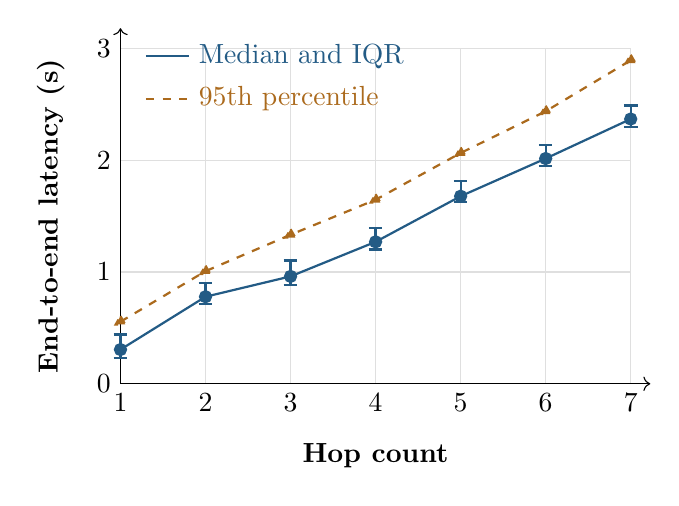
\begin{tikzpicture}[x=1.08cm,y=1.42cm,font=\normalsize]
    \draw[gray!25,xstep=1.08cm,ystep=1.42cm] (1,0) grid (7,3);
    \draw[->] (1,0) -- (7.23,0);
    \draw[->] (1,0) -- (1,3.18);
    \foreach \x in {1,...,7} \node[below] at (\x,0) {\x};
    \foreach \y in {0,...,3} \node[left] at (1,\y) {\y};
    \node[below,font=\normalsize\bfseries] at (4,-.45) {Hop count};
    \node[rotate=90,font=\normalsize\bfseries] at (.18,1.5) {End-to-end latency (s)};
    \foreach \x/\lo/\hi in {1/.2315/.44075,2/.717/.903,3/.88575/1.10325,4/1.2015/1.39075,5/1.62325/1.8135,6/1.95075/2.139,7/2.298/2.48875} {
      \draw[jbblue,thick] (\x,\lo) -- (\x,\hi);
      \draw[jbblue,thick] (\x-.08,\lo) -- (\x+.08,\lo);
      \draw[jbblue,thick] (\x-.08,\hi) -- (\x+.08,\hi);
    }
    \draw[jbblue,thick] plot[mark=*] coordinates {(1,.306)(2,.7785)(3,.9605)(4,1.2695)(5,1.6775)(6,2.0145)(7,2.368)};
    \draw[jbamber,thick,dashed] plot[mark=triangle*] coordinates {(1,.555)(2,1.007)(3,1.333)(4,1.646)(5,2.064)(6,2.437)(7,2.893)};
    \draw[jbblue,thick] (1.30,2.93) -- (1.80,2.93) node[right]{Median and IQR};
    \draw[jbamber,thick,dashed] (1.30,2.55) -- (1.80,2.55) node[right]{95th percentile};
  \end{tikzpicture}
  \caption{Hop latency at a 500\,ms drain interval. All 50 posts reached hop seven.}
  \label{fig:chain}
\end{figure}

The default HTTP limiter rejected 2,709 of 3,000 invalid inputs. With the limit raised, 2,593 reached bad-signature rejection. All 3,000 malformed requests returned HTTP 400, 1,000 exact repeats returned existing receipts, and 1,000 nonce replays on non-idempotent writes returned HTTP 409. These runs yielded zero profiled writes. The five-peer gRPC run rejected 500 invalid-signature frames. Over-quota traffic blocked two peers and caused 15 peer-state writes with zero envelope inserts.

At concurrency 1, 4, 16 and 32, all 200 valid posts per setting reached the local projection. Throughput was 29, 27, 9 and 6 requests/s, with p95 latencies of 49, 353, 4{,}132 and 12{,}587\,ms. Docker application memory snapshots ranged from 108 to 181\,MiB after these batches, MongoDB used 150--345\,MiB, and Redis stayed below 9.5\,MiB. The eight-node application containers used 77--111\,MiB each, with a sampled CPU maximum of 21.18\%. These samples give no estimate of peak RSS or disk footprint.

The encoding ratios exclude transport and do not imply equivalent functionality or interoperability.

On the constrained link both systems delivered 20/20 posts. Jagoo Bahee recorded a 521\,ms median (95\% CI 394--586\,ms) and 1{,}846 sender-interface bytes/post. The minimal AP inbox recorded 155\,ms (95\% CI 145--161\,ms) and 1{,}278 bytes/post. Application memory snapshots were 88--92\,MiB versus 9--14\,MiB. The inbox excludes the Mastodon application and worker stack. With inbound blocked, periodic pull recovered 10/10 posts (median 1.046\,s), while inbox push delivered 0/10. With its listener disabled, an outbound-only node pulled 10/10 and pushed 10/10 in a separate run.

\section{Discussion and Limitations}
\label{sec:limits}

\textbf{Testbed validity.} All experiments ran on a single physical machine over virtual networks using Docker, and this is the paper's main limitation. Every node shared one kernel, clock, CPU and storage subsystem. The shared clock makes timestamp subtraction valid in this setup. Physical routers, BGP reconvergence, NAT, DNS failures, variable MTUs, and wireless links introduce conditions outside this evaluation. A deployed bridge also needs independent links, routing policy, credentials, power, and an operator.

\textbf{Access and subscriber isolation.} The system assumes that nodes on the same network can communicate with each other or reach a shared bridge. However, some Wi-Fi networks and ISPs block direct communication between customers while still allowing them to access the provider's gateway. If this restriction exists on every available path, nodes cannot connect to each other or reach the bridge. In that situation, federation completely stops, and only local services continue to work. The current prototype has no alternative non-IP method for communication in this situation.

\textbf{Network adversary.} A network operator can do multiple things. They can identify endpoints or RPC traffic, block IP addresses or SNI values, track communication timing, isolate a node, or pressure a bridge operator. Source-address binding only chooses which network connection to use; it does not hide the traffic. There is also one important failure case: \textbf{protocol whitelisting}. In this situation, normal domestic Internet routing still works, but deep packet inspection allows only approved protocols. Since the federation uses a distinctive, non-standard protocol on a specific port, it could be blocked immediately, regardless of how strong our signatures are. Possible solutions include running federation over normal HTTPS, changing endpoints regularly, or using pluggable transports. However, none of these solutions has been implemented or tested in this work.

\textbf{System and application limits.} Signatures prove who published something, but they do not prove that the content is truthful or safe. A legitimate key can still be used to publish harmful content or generate a large amount of traffic. Since the admission cost is handled by the origin, an origin operator can generate as many free proofs as needed for its own users. This means that protection against abuse depends largely on the policies of the weakest origin in the peer group. The per-peer rate limits provide the main layer of protection in this case. Other problems remain open, such as stolen keys, exposed metadata, large-scale moderation, recovering from revoked keys, running out of storage, and coordinated fake identities (Sybil attacks). Local RFC 6962 consistency proof generation and verification are implemented \cite{rfc6962}, with proof retrieval over HTTP. Peer gRPC growth verification, cross-observer fork detection under partition, and automated ALS comparison of heads remain open. Most importantly, a receipt only proves what the system \textbf{accepted and acknowledged}. If an operator simply refuses to accept something, no receipt is created. The system therefore cannot prove a refusal to admit content.

\textbf{Evaluation limits.} We ran no independent multi-host, wide-area, multi-day, or real-shutdown trials. Inter-host timestamp comparisons would require measuring clock skew. The x86 CPU and memory snapshots establish neither resource-exhaustion thresholds nor performance on single-board computers.

\textbf{Ethics.} The controlled tests used synthetic content on isolated private networks. The encoding comparison sampled public activities. However, a real deployment could put bridge operators and users at legal or physical risk because a visible relay can be identified by the network hosting it. Therefore, the system should not be deployed in a hostile environment without first assessing local threats, getting informed consent, minimizing collected data, and reviewing the deployment with the affected community.

\section{Conclusion}

On the single-host testbed, canonical signed objects, one admission path for local and federated traffic, caller-initiated recovery and a trusted validating relay delivered all 20 dependency chains after the exchange cut. Median bridged post latency was 1.732\,s. The controlled inbox comparison shows different latency and delivery behaviour under loss and blocked inbound access. Multi-host evaluation, resource-exhaustion tests, peer verification of growing logs, and a fallback for total loss of IP connectivity remain open.

\bibliographystyle{IEEEtran}
\bibliography{iccit2026-paper-pre-references}

\end{document}
